\chapter{目标检测与位姿估计方法研究}
\label{cha:detect_pose_estimation}
\section{引言}
\label{sec:detect_intro}
本文在第~\ref{cha:model_based_tracking}~章中研究了基于目标物体三维模型的位姿追踪算法,该算法追踪精度高,鲁棒性强,但追踪系统在第一帧中需要人为给定目标物体相对于相机的位姿关系,即初始化过程。
该缺陷导致算法无法自动对目标实现追踪,增加了算法运行的人力成本。并且初始化的精度将影响后续追踪的精度,若初始化误差较大,模型边缘将有可能误匹配至背景边缘中,导致追踪失败。本章将针对该问题
研究目标物体的检测与姿态估计方法,以实现追踪算法的自动初始化,提高初始化精度。且在追踪算法出现较大误差后,能够利用检测与位姿估计算法进行重新初始化,
该策略能够应对目标物体消失或大面积被遮挡的情况,当物体再度出现在相机视野内时,算法能够及时初始化新的追踪过程,实现对目标的再度追踪。

已有较多方法能够实现目标检测与姿态估计,其中利用特征点匹配定位的方法已经取得了不错的效果\cite{PiImplementation3DPose},如图~\ref{fig:chap04:detect_feature_pose_estimation}~所示。该类方法首先对物体表面特征点进
行提取并保存,之后对特征点进行物体模型上的定位,以得到特征点在三维物体上的位置关系;
最后通过输入图像进行特征点匹配以检测目标物体,并获得特征点的图像坐标,通过特征点的模型位置与图像坐标的关系结算目标物体位姿,即解~PnP~问题。该方法检测准确度高,位姿解算精度符合本文初始化要求,但其必须依靠
目标表面特征点,因此并不适用于贫纹理目标。Eric~等人\cite{BrachmannUncertaintyDriven6DPose2016}于~2016~年提出的基于像素点分类的方法能够对任意目标物体实现检测与位姿估计,但其方法需要准备大量的要有位姿真值的图片数据,前期标注成本较高;
且易受与目标物体颜色相同的背景物的干扰,因此常出现误差较大的情况,仍不适用于本文的初始化需求。

为实现自动初始化的追踪算法,本文将针对贫纹理物体研究其检测以及姿态估计的方法。提出基于~DCM~张量作为特征图像的随机森林分类检测器,通过对~DCM~张量图进行特征提取训练随机森林分类器,之后
对输入图片进行滑窗检测以确定目标物的图像位置。之后使用回归以及模板匹配的方法
获得目标相对相机的位姿关系,实现高精度的检测以及姿态估计系统。最后整合该系统至前文所研究的目标追踪系统中,实现自动初始化,并使用追踪失败后的重新初始化策略提高追踪系统的鲁棒性。

\begin{figure}[t] %[h]
    \centering%
    \subcaptionbox{特征点提取\label{fig:chap04:detect_feature1}}{%    
      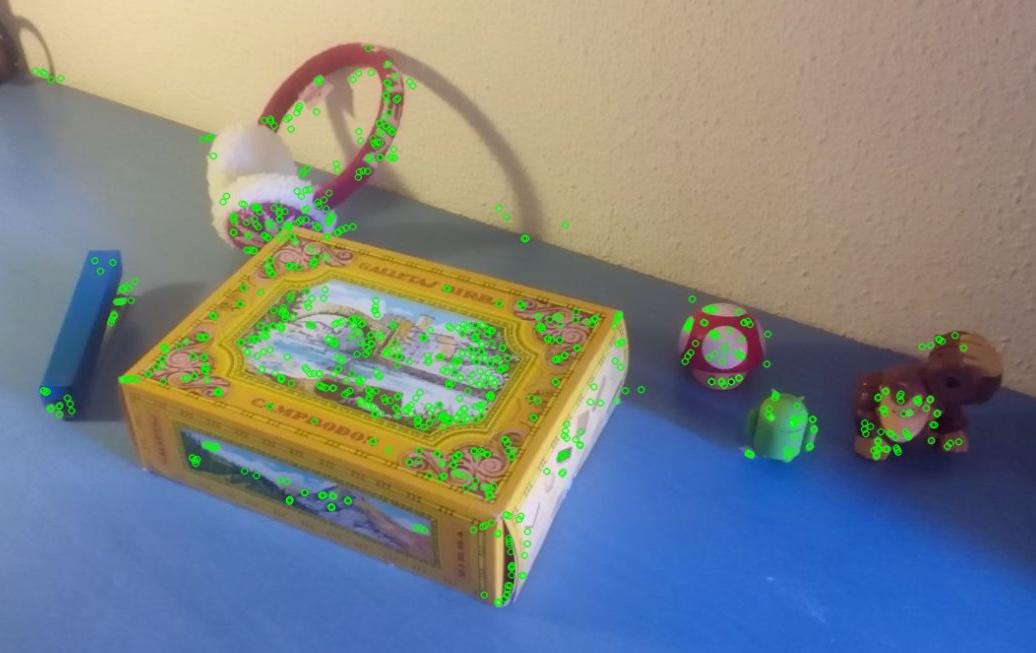
\includegraphics[height=4cm]{feature_detect1}\hspace{2em}}%\vskip0.2cm
    \subcaptionbox{确定特征点模型位置\label{fig:chap04:detect_feature2}}{%  
      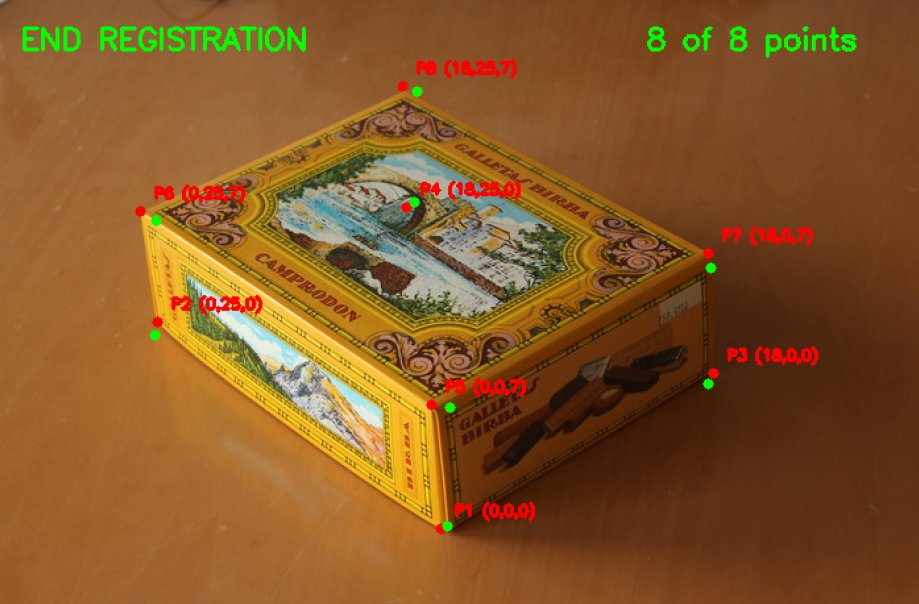
\includegraphics[height=4cm]{feature_detect2}}\vskip0.2cm
    \quad
    \subcaptionbox{特征点匹配\label{fig:chap04:detect_feature3}}{%  
      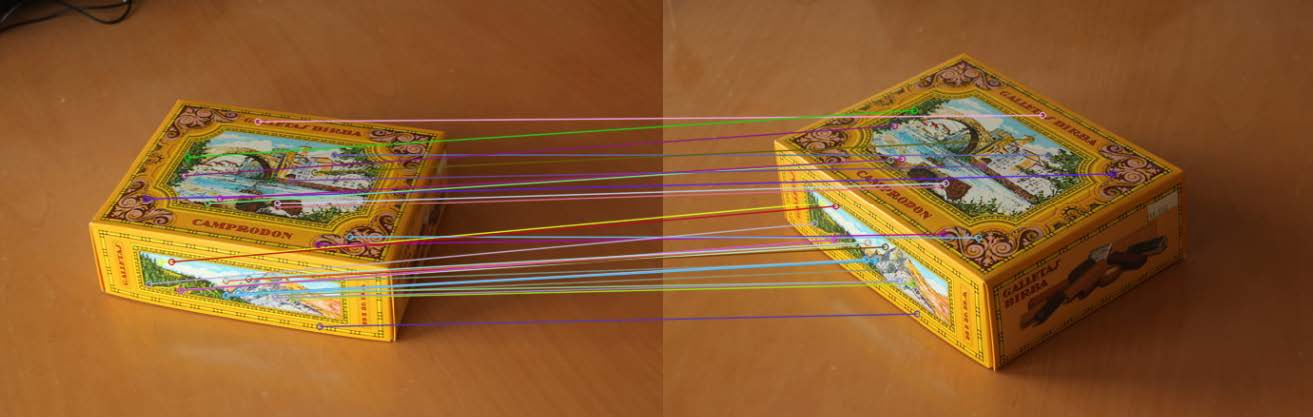
\includegraphics[height=4cm]{feature_detect3}}%\vskip0.2cm
    \caption{基于特征点的定位与姿态估计算法}
    \label{fig:chap04:detect_feature_pose_estimation}
  \end{figure}


\section{基于~DCM~张量的目标检测方法}
\label{sec:DCM_object_detect}
由于贫纹理目标无法使用特征点匹配的方法进行检测,因此本文研究基于模型边缘的检测方法。使用章节~\ref{sec:Tensor calculation}~中提出的方向倒角匹配张量计算目标边缘特征,利用随机森林对特征进行学习。
检测阶段对输入图像进行滑窗分割,进而对每一个分割的图片进行特征提取,并使用已训练的随机森林对不同图片的特征进行分类,判断是否包含目标物体。该方法相比特征点匹配的方法适用范围更广,并且能够对单一目标在不同姿态下进行区分,
检测阶段就对目标姿态进行粗分类。

\subsection{特征提取}
\label{sec:NPD}
贫纹理目标无法进行特征点提取,因此本文使用~DCM~张量计算匹配最近点图像,并使用归一化像素差特征对图像进行特征提取,以训练分类检测器。DCM~张量代表边缘图像中所有像素点的方向与距离的最近匹配关系,
由于对方向进行了离散化\footnote{本文将边缘方向离散化为~60~个角度范围},因此单张原始图像的~DCM~张量包含了各离散边缘的匹配关系。本文首先对~DCM~张量进行整合,得到匹配最近点图像,该图像中
所有像素点的灰度值代表该点在各方向中的匹配最小值。如图~\ref{fig:chap04:matching_min_point}~所示,通过追踪算法得到的物体~DCM~数据库,计算物体的匹配最近点图像,该图像包含了目标的边缘匹配信息,提取图像特征以检测目标。
使用多分类的检测器不仅能够检测出目标的图像位置,还能对姿态进行粗分类,以便后续姿态计算。

\begin{figure}[t] %[h]
  \centering%
  \subcaptionbox{原始追踪图像\label{fig:chap04:tracking_img}}{%    
    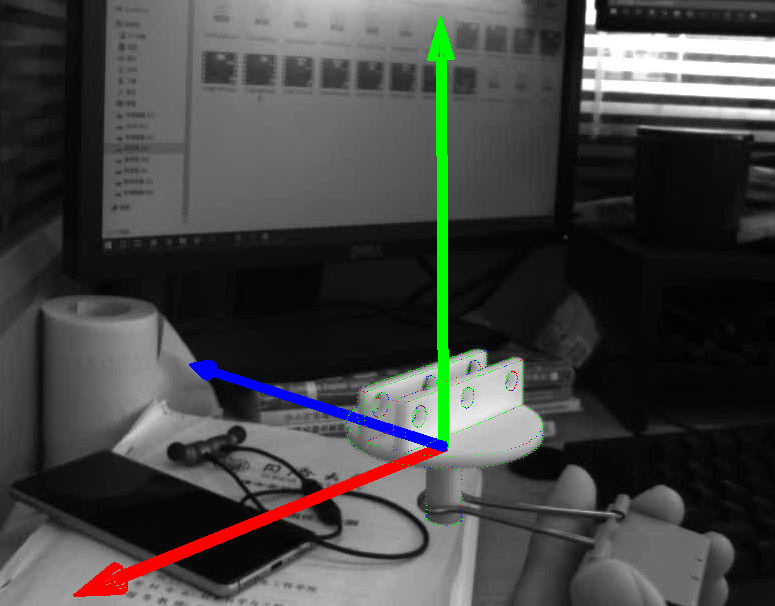
\includegraphics[height=3.8cm]{san_tracking}\hspace{1em}}%\vskip0.2cm \hspace{2em}
  \subcaptionbox{各方向~DCM~张量\label{fig:chap04:60dire_DCM}}{%  
    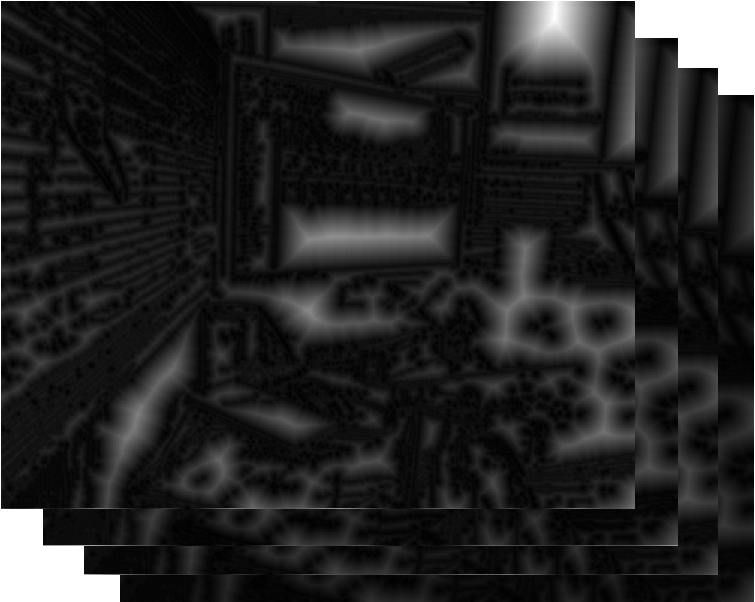
\includegraphics[height=3.8cm]{60_DCM}\hspace{1em}}%\hspace{2em}
  \subcaptionbox{匹配最近图\label{fig:chap04:min_matching}}{%  
    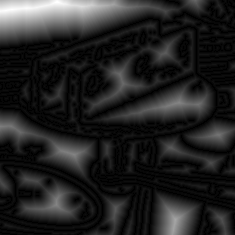
\includegraphics[height=3.8cm]{san_tensor}}%\vskip0.2cm   
  \caption{匹配最近图计算}
  \label{fig:chap04:matching_min_point}
\end{figure}

通过追踪算法能够确定目标物体在图像中的位置,按照该位置对匹配最近图进行分割,如图~\ref{fig:chap04:min_matching}~所示,以此作为特征提取的输入图片。
在分割后的匹配最近图中能够明显观察到目标的轮廓信息,其中每个像素点的灰度值代表该点在~60~个离散方向上的最小~DCM~距离。距离边缘点远的像素点灰度值高,距离边缘点近的点灰度值低。
该图像能够直观反应物体轮廓信息,便于利用提取特征方法,判断图像中是否含有目标物体。

本文使用归一化像素差特征(Normalized Pixel Difference,简称~NPD)对匹配最近图进行特征提取。NPD~特征用于描述图像中所有像素点间的差异性,该差异定义为函数~$f(x,y)$,具体描述如式~(\ref{equ:chap4:NPD})。
\begin{equation}
  \label{equ:chap4:NPD}
    f(x,y)=\frac{x-y}{x+y}
\end{equation}
其中~$x,~y\geq 0$~为图像中任意两个像素的像素值,且规定~$f(0,0)=0$。由于~NPD~表达的是两个像素之间的相对差异,相同像素间没有差异,因此规定为~0。如图~\ref{fig:chap04:NPD_cal}~所示为~NPD~特征的取值示意图,其中~x,y~轴
分别代表两个像素点的灰度值。NPD~特征具有许多较好的属性:(1)~像素尺度不变性,与像素差
绝对值~$|x-y|$~相比,NPD~特征的波动范围更窄,即不会由于某一个像素点的灰度值较高或较低而导致所有关于该点的~$f(0,0)$~都偏高或偏低;(2)~反对称性,使用~$f(x,y)$~或~$f(y,x)$~就足以表达整个空间,使特征
空间减少;(3)~对光照的强鲁棒性,由于~NPD~是两个像素的差值,受像素本身的影响较小,发生光照变化时,像素点的整体灰度值都会受到相似的影响,该变化对于像素的插值影响较低,因此该特征对光照具有较强的鲁棒性;
(4)~特征维度较大,对于~$s*s$~的图像块(向量化为~$p*1$~维,其中~$p=s*s$),计算所有像素对~$x_i,y_j$~的~NPD~特征~$f(x_i,y_j),~1\leq i<j\leq p$,该特征的维度为~$d=p*(p-1)/2$。比如大小为~$24*24$~的图片,NPD~特征维度为
~$(24*24)*(24*24-1)/2=165600$,对于单张图片,其特征维度已经超过~16~万,因此~NPD~特征是一种计算简单但特征维度巨大的特征提取算法,使用该算法虽然能够有效提取像素点间的差异特征,但特征维度过大会在训练时导致速度过慢或者内存溢出的问题,
因此本文综合考虑特征训练的分类结果以及训练时的硬件成本和时间成本,使用更小的灰度图片进行特征提取,其中使用~$20*20$~的灰度图像,特征维度下降~$51.81\%$,使用~$15*15$~的灰度图像,特征维度下降~$84.78\%$,如图~\ref{fig:chap04:NPD_feature_extra}~为
三张图片进行~NPD~特征提取后的前~500~维特征的示意图,其中不同颜色代表不同图片。特征维度的下降意味着特征量的降低,
由此对训练结果的影响将在后续进行详细比较。最后,NPD~特征~$f(x,y)$~归一化在~$[-1,1]$~之间,它的有界属性使得该特征适用于基于树分类器中的直方图合并和阈值学习。

\begin{figure}[t] %[h]
  \centering%
  \subcaptionbox{NPD~特征取值示意图\label{fig:chap04:NPD_cal}}{%    
    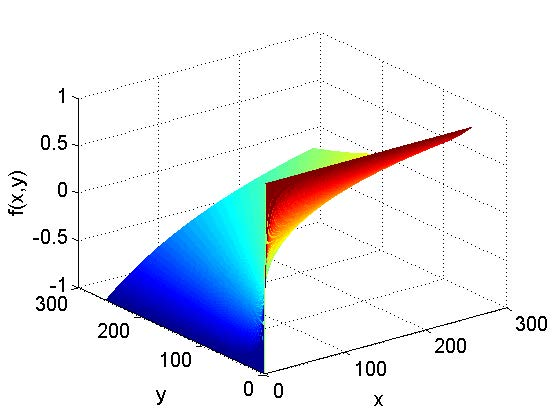
\includegraphics[height=5cm]{NPD_cal}\hspace{1em}}%\vskip0.2cm \hspace{2em}
  \subcaptionbox{多张图片特征空间\label{fig:chap04:NPD_feature_extra}}{%  
    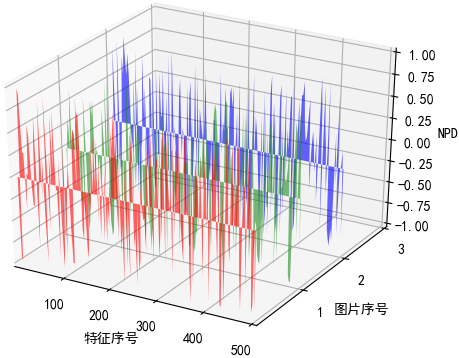
\includegraphics[height=5cm]{NPD_feature_show}}%\hspace{2em}  
  \caption{NPD~特征示意图}
  \label{fig:chap04:NPD_feature}
\end{figure}

\subsection{决策树分类算法}
\label{sec:random_forest}
决策树\cite{NasrabadiPatternRecognitionMachine2007,WangjueJiQiXueXiJiQiYingYong2006}~(Decision Tree)~是机器学习中一个常用的分类算法。以本文目标检测为例,将不同物体分为不同的类别,首先判断
是否为目标物体,再对目标物体进行类别分类。假设需要分类的贫纹理工件有三类,则本次为三分类任务。而决策树是处理“是”与“否”的二分类结构,可以先将两种工件分为一个大类,而将另一种工件单独为一个类,先进行大类区分,
再对小类进行二分,直到寻找到单独对应的小类为止。以此类推,虽然单次划分类别有限,但可以通过级联分类的方法进行多分类。决策树,顾名思义,是模拟树结构来进行决策的,这与人做判断时的逻辑过程类似。比如,在判断
一张图片是否含有目标物体时,会进行一系列的判断:“是否有特定长度的边缘?”、“是否有正方形的的平面区域?”或者“是否有三个圆形的孔?”。如果以上判断都满足,则可以判断图像中包含目标物体,如果不能,则再继续判断。
其中每个判断问题都是对某个属性的测试,每个测试得到的结果即最终结论或是进一步需要判断的问题,当前判断的范围仅限定在上一次的决策结果之内,每一次判断都将使得最终的结果进一步缩小。

决策树包含一个根节点、多个内部分裂节点和叶节点。根节点包含了整个样本集合。从根节点出发,到每个叶节点结束,每一条支路对应于一个决策序列。叶节点存放着决策判断的结果,其他每个分裂节点则是对某一个属性的测试;
根据属性测试的结果,每个分裂节点包含的样本合集被划分到对应的子节点中;决策树学习的目的是为了产生一棵能应对未知数据的具有强泛化能力的判别模型,其流程遵循“分而治之”的策略\cite{ZhouzhihuaJiQiXueXi2016},如算法~\ref{alg:tree_train}~所示。

\begin{algorithm}[H]
  \caption{[Node]=$Tree(D,A)$}
  \label{alg:tree_train}
  \begin{algorithmic}[1]
    \Require{训练集 $D={(x_1,y_1),(x_2,y_1),\dotsc ,(x_n,y_m)}$;属性集 $A={a_1,a_2,\dotsc ,a_m}$}
    \State 生成节点~Node.
    \If{~$D$~中样本全属于同一类别~C~}
      \State 将~Node~标记为~$C$~类叶节点 \Return
    \EndIf
    \If{~$A=\varnothing $~\textbf{OR}~$D$~中的样本在~$A$~上的取值相同}
      \State 将~Node~标记为叶节点,其类型标记为~$D$~中样本数最多的类 \Return
    \EndIf
    \State 从~$A$~中选择最优划分属性~$a_*$~.
    \For{$a_*$~的每一个值~$a_*^v$~}
      \State 为~Node~生成一个分支;令~$D_v$~表示~$D$~中在~$a_*$~上取值为~$a_*^v$~的样本子集。
      \If{~$D_v=\varnothing $~}
        \State 将分支节点记为叶节点,类别标记为~$D$~中样本最多的类 \Return
      \Else 
        \State 以~$Tree(D_v,A\{a_*^v\})$~为分支节点。
      \EndIf
    \EndFor
    \\
    \Return {以~Node~为根节点的一棵决策树}
  \end{algorithmic}
\end{algorithm}

决策树的训练就是从给定的训练数据集(本文中为不同工件在不同姿态下的匹配最近图)中学得一个模型用以对新的输入
样本进行分类。在决策树生成的过程中,学习的终止条件有三个:第一,当前节点中的样本都是同一类别,不需要继续分类;第二,当前的属性集为空或者样本在所有的属性上取值一样,不能继续划分;
第三,当前节点中无样本,不能划分。

决策树生成过程中,最重要的一步就是选择最优划分属性。通过不断对样本的划分,最终使得分支节点的样本都属于同一种类,即使节点中的样本纯度达到最高。决策树的属性划分是伴随着决策树的改进过程提出的,
其判断准则主要有三个:信息增益、信息增益率和基尼指数,分别是对应于~ID3,~C4.5和~CART~等决策树生成算法。下面对主要的属性划分方法进行介绍。

\noindent\textbf{信息增益:}衡量样本集合内数据纯度的一个常见指标。它假设当前样本~$D$~中第~$k$~类样本占比为~$p_k(k=1,2,\dotsc ,|\upgamma|,~|\upgamma|$为本次分类的类别总数),则可以定义~$D$~的信息增益熵为:
\begin{equation}
  \label{equ:chap4:ent}
  Ent(D)=-\sum_{k=1}^{|\upgamma |} p_k \log_2 p_k
\end{equation}
$Ent(D)$~的值越小,则代表相应的~$D$~的纯度越高。假设样本集~$D$~中的一个离散属性~$a$~有~$V$~个可能取值,那么用该属性来划分空间会产生~$V$~个分裂节点,其中第~$v$~个分裂节点中包含的是样本集~$D$~中所在
属性~$a$~上取值为~$a^v$~的样本数据,记作~$D^v$。信息增益,如式~(\ref{equ:chap4:gainDa})~所示,是在此基础上,针对所有属性~$a$~的划分在整个样本空间的比重系数。信息增益越大,表示使用该属性划分带来的分支纯度越高。
\begin{equation}
  \label{equ:chap4:gainDa}
  Gain(D,a)=Ent(D)-\sum _{v=1}^V \frac{|D^v|}{|D|}Ent(D^v)
\end{equation}

\noindent\textbf{增益率:}使用信息增益作为评价标准会造成倾向于取值较多的属性(即~$v$~较大),比如每一个样本都具有独一的编号属性,若通过编号划分将使得每一个子节点仅包含一个样本,此时按照编号划分后的
信息增益最大,分支纯度最高,但选择编号作为分类指标将会使得样本泛化能力降低,导致过拟合。为了消除该缺陷,在信息增益的基础上增加了一个抑制系数~$IV$,其定义如下:
\begin{equation}
  \label{equ:chap4:IVa}
  IV(a)=-\sum_{v=1}^V \frac{|D^v|}{|D|}\log_2 \frac{|D^v|}{|D|}
\end{equation}
若对于属性~$a$,其取值~$v$~数量较多,且对应每一种取值的样本数量~$|D^v|$~较小时,该抑制系数的取值就会较大。将~$IV$~加入式~(\ref{equ:chap4:gainDa})~中,以得到增益率的计算方法,如式~(\ref{equ:chap4:zengyi})。
改进后的策略相比于信息增益将更加偏好于选择取值数目较少的属性。
\begin{equation}
  \label{equ:chap4:zengyi}
  Gain_r (D,a)=\frac{Gain(D,a)}{IV(a)}
\end{equation}

\noindent\textbf{基尼系数:}采用的方式与以上两种不同,它用来度量两极分化程度,是熵的一阶近似。基尼值~$Gini(D)$~用于衡量样本的纯度,直观上
理解,其反映了从数据集~$D$~中随机抽取两个样本,其类型标记不一致的概率。因此基尼值越小,样本纯度越高,计算如式~(\ref{equ:chap4:gini})。
\begin{equation}
  \label{equ:chap4:gini}
  Gini(D)=\sum_{k=1}^{|\upgamma |}\sum_{k'\neq k}p_k p_{k'}=1-\sum_{k=1}^{|\upgamma|}p_k^2
\end{equation}
基于基尼值计算基尼指数,选择基尼指数最小的属性作为最优划分属性,计算如式~(\ref{equ:chap4:gini_index})。
\begin{equation}
  \label{equ:chap4:gini_index}
  Gini\_index(D,a)=\sum_{v=1}^{V}\frac{|D^v|}{|D|}Gini(D^v)
\end{equation}

本文采用~NPD~特征作为决策树划分的属性,区别于“是”与“否”类型的属性,NPD~特征的取值范围非常大,因此不能直接运用以上的属性划分规则。针对这个情况,本文采用二分法对~NPD~特征进行处理,以减少决策树的分支。
假设样本集合~$D$~中的一个属性~$a$~是连续型属性,$a$~的取值有~$n$~种情况,则将属性~$a$~的所有取值按照升序排列~$\{a_1,a_2,\dotsc,a_n\}$。设置划分点~$t$~可将样本集合分为~$D_t^+$~和~$D_t^-$,
$D_t^+$~中包含在属性~$a$~上取值大于~$t$~的样本,$D_t^-$~中为属性~$a$~上取值小于~$t$~的样本。因此在决策树学习过程中,不仅需要对划分属性进行选择,还需要对属性的取值和划分点进行学习。

\subsection{目标多位姿分类检测器}
\label{sec:object_detector}
本文将根据决策树分类算法,使用随机森林对贫纹理物体进行多分类检测。随机森林是一个包含许多决策树的分类器,该分类器最早由~Leo Breiman\cite{BreimanRandomForests2001}~提出,并得到广泛的应用。
随机森林是一种集成学习,相较于决策树这样的单一学习器,它能有效提升整体的泛化能力。在随机森林中,对于每棵决策树的每个分裂节点,先从该分裂节点的候选属性集(假设有~$m$~个)中选择一个包含~$k$~个属性的子集,然后
再从该子集中选择一个最优划分属性。$k$~的大小控制了随机的程度,若~$k=m$~则选择了所有属性,与原始的决策树相同。在属性维度较大的情况下,建议的~$k$~值为~$\log_2 m$。随机森林的每一棵决策树之间是没有关联的,
每一棵决策树所选择的特征也是不同的,通过随机选择特征来对训练样本进行层级划分,当节点的样本纯度或决策树深度达到上限时则停止划分。在完成训练后,每一棵决策树都将对新输入的样本进行判断,以得到每一棵决策树的分类结果,
最后通过统计所有输出中占比最大的结果作为随机森林的输出。
\begin{figure}[b] %[h]
  \centering%
  \subcaptionbox{二分类\label{fig:chap04:double_dir}}{%    
    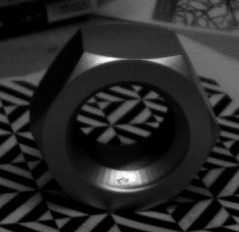
\includegraphics[height=4cm]{item1zhong}\hspace{1em}%\vskip0.2cm
    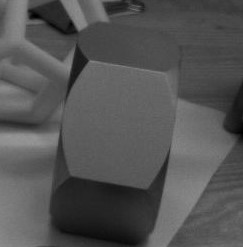
\includegraphics[height=4cm]{item2zhong}}\vskip0.2cm
  \quad
  \subcaptionbox{三分类\label{fig:chap04:triple_dir}}{%  
    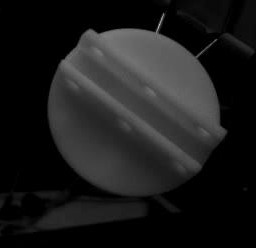
\includegraphics[height=4cm]{item2ding}\hspace{1em}
    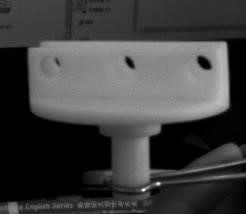
\includegraphics[height=4cm]{item2ce}\hspace{1em}
    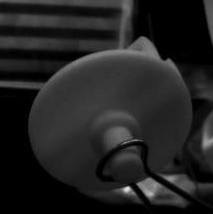
\includegraphics[height=4cm]{item2di}}%\vskip0.2cm
  \caption{目标检测分类}
  \label{fig:chap04:rf_obj_det_pose}
\end{figure}

该随机森林首先判断场景中是否有目标物体,若存在目标物体则判断是哪一类目标物,确定目标物类型后再对其姿态进行粗分类。也即不同的目标物体在不同姿态下对应的是不同的类别。如图~\ref{fig:chap04:rf_obj_det_pose}~所示,通过对训练样本的划分,将
不同物体的姿态进行粗分类。根据模型的对称情况,进行分别处理,如图\ref{fig:chap04:triple_dir}所示,由于该工件在顶面、侧面、底面轮廓信息差距较大,因此将位姿粗分为三类;而对于图~\ref{fig:chap04:double_dir}~所示的工件,存在较强的对称关系,其在顶面和底面的
轮廓信息基本相同,因此只分为两类。由于目标物体在不同粗分类位姿下轮廓信息差距较大,因此能够将同一个物体在不同粗分类位姿下的特征作为随机森林里的不同类别进行区分。在目标检测阶段对位姿进行粗分类能够有效减少姿态估计时的
模板数量,提高初始化的成功率以及准确性。本文使用由~800~棵决策树构成的随机森林,并且设定每棵树的最大深度为~10~层。使用第~\ref{cha:dataset}~章中准备的匹配最近图数据库对随机森林进行训练,其中包含~4~种目标物体,为保证模型的抗干扰性,本文还在训练
样本中加入了~9000~余张负样本,负样本同样截取自真实视频中,负样本的图片尺寸与正样本相同。

训练过程分为四个步骤。首先由于数据库图片的大小都不相同,因此导致~NPD~特征的尺度也会存在较大差异,无法提取出共性特征,因此先将数据库图片的大小进行统一,通过将一定范围内的像素灰度值进行平均值整合以将所有数据库图片
大小压缩为~15*15。其次对所有压缩后的图片进行~NPD~特征提取,单张图片的特征维度为~25200,并且数据库图片较多,因此计算量较大本文利用线程池的方法对特征进行提取\footnote{特征提取:https://github.com/CNchence/Tensor\_random\_forest\_sklearn},
极大程度加快了特征提取的速度。随后将数据库中保存的分类真值加入到特征矩阵中,得到完整的随机森林训练数据。最后使用机器学习库对特征进行分析并完成所有分类决策树的学习与构建,得到完整的目标多位姿分类检测器,
由于特征量巨大,本文使用基于~Python~的~sklearn~机器学习库完成训练,该库数据导入导出速度较快,且能够通过指定参数的方式对随机森林的结构以及特征的选用进行灵活的设置,所以采用该库完成随机森林的构建。

检测阶段,使用滑窗的方式对输入图片进行检测,即通过滑窗选定一定区域的图片进行剪切,使用随机森林对剪切后的图片进行分类判定。首先选定一系列滑窗的大小,滑窗的步进设定为其大小的~10\%。之后将剪切后的图片压缩到~15*15,并进行~NPD~特征提取。
最后将提取后的特征作为随机森林的输入,以得到该剪切区域的分类结果。随机森林的输出由所有决策树的分类结果得到,当超过~80\%~的决策树输出都相同时,才将该结果作为随机森林的结果进行输出,否则分类结果为背景,即不包含
目标物体。



\section{基于回归与模板匹配的位姿估计方法}
\label{sec:template_matching}
通过目标检测,得到物体在相机成像平面中的二维图像坐标,为完成位姿初始化,还需通过图像信息解算物体相对于相机的三维位姿。本文研究基于回归树的目标平移向量估计方法,通过目标在图像中的二维坐标以及模型信息确定其相对于相机坐标系的平移向量。
由于本文在检测阶段就对不同目标物体进行了姿态粗分类,因此在得到平移向量~$\textrm{T}$~后,针对不同的分类类型,构建匹配模板库。之后通过第~\ref{cha:model_based_tracking}~章研究的模型与边缘图像的对齐算法以得到物体相对于相机坐标系的精确
旋转矩阵~$R$,以完成自动初始化算法。

\subsection{回归树算法}
\label{sec:regression_trees}
回归树属于决策树的一种,与分类树类似,通过对节点样本的不断划分以在叶节点得到判定的结果。回归树是通过递归分区构建得到的,该方法按照样本的特征不断将数据拆分为两个分区,直到分区内的数据波动范围低于一定阈值为止。此时
该分区被设定为叶节点,其中所有数据的均值作为该叶节点的输出。
由于回归树是处理连续值的预测问题,因此其输出是一个实数,这区别于分类树的输出,因此回归树节点的划分规则与分类树也完全不同,前文所述的信息增益、增益率以及基尼指数都不再适用。

回归树的划分规则就是要让两个分区的所有样本与分区代表值的平方差最小。假设选择~$j$~作为当前划分的特征,它的取值~$s$~为划分点,即可得到两个划分区域:
\begin{equation}
  \label{equ:chap4:huafenquyu}
  \left\{
    \begin{aligned}{}
      R_1(j,s) = \{x|x_j\leq s\} \\
      R_2(j,s) = \{x|x_j > s\}
    \end{aligned}
    \right.
\end{equation}
寻找划分特征~$j$~以及切分点~$s$~使得两个区域的损失函数最小,如式~(\ref{equ:chap4:regre_tree_loss})~。
\begin{equation}
  \label{equ:chap4:regre_tree_loss}
  \min_{j,s}\left[ \min_{c_1}\sum _{x_i \in R_1(j,s)} (y_i - c_1)^2 + \min_{c_2}\sum _{x_i \in R_2(j,s)} (y_i - c_2)^2\right]
\end{equation}

其中~$c_1,~c_2$~表示划分后的两个分区的代表值,也即分区中所有样本值~$y$~的平均值,如式~(\ref{equ:chap4:daibiaozhi})。若当前分区作为叶子节点,则其输出值也即该分区的代表值。
\begin{equation}
  \label{equ:chap4:daibiaozhi}
  \left\{
    \begin{aligned}{}
      c_1 = ave(y_i | x_i \in R_1(j,s)) \\
      c_2 = ave(y_i | x_i \in R_2(j,s))
    \end{aligned}
    \right.
\end{equation}

\subsection{基于回归树的平移向量估计方法}
\label{sec:T_regression}
目标物体相对于相机坐标系的平移向量代表物体坐标系原点相对于相机坐标系原点的三维空间位置关系,其由相机坐标系的三轴平移向量构成,如式~(\ref{equ:chap4:T})。
\begin{equation}
  \label{equ:chap4:T}
  \textrm{T} = \left[\begin{matrix} t_x\vec{i} \\  t_y\vec{j} \\ t_z\vec{k} \end{matrix} \right]
\end{equation}

式中~$t_x, t_y, t_z$~分别代表物体坐标系原点在相机坐标~$x,y,z$~轴上的坐标,$\vec{i},\vec{j},\vec{k}$~分别为相机坐标系~$x,y,z$~轴上的单位向量。假设相机坐标系原点为~$O_c$~,
物体坐标系原点为~$O_c'$,可得:
\begin{equation}
  \label{equ:chap4:point_T}
O_c' = O_c + \textrm{T}
\end{equation}

$t_z\vec{k}$~代表物体坐标系原点在相机坐标中的深度,然而单目灰度相机无法直接提取场景深度信息。当已知目标物体模型时,能够根据相机投影模型以及图像坐标系中物体的尺寸对其深度进行估计。
但该方法需要在图像中寻找到预先设定的物体表面特征点以计算其图像尺寸,且对于不同物体的不同位姿,都需要在图像中定位至少两个点,这对于本文所选择的贫纹理对象而言十分困难,且深度的估计需要进行标定,
这也将加大该方法的难度以及成本。因此本文研究使用回归树的方法对目标物体的深度进行估计,具体方法是通过检测框的大小以及图像位置对深度进行估计。当物体模型固定之后,其图像大小与其相距相机光心的距离存在
耦合关系,因此通过检测框的顶点坐标以及检测框的大小作为特征,目标的深度作为估计值,构造回归树。
前文已由追踪算法得到大量真实图片的检测框信息以及平移向量的真值数据,使用该数据库对回归树进行训练以估计物体深度。通过该方法得到的~$t_z$~相比相机模型估计的方法鲁棒性更高,在不同物体的不同位姿下都能较为准确地对深度进行估计。

目标物体相对于相机的平移向量与检测框的图像位置和大小有关,且对于模型与所处位姿的不同存在很大差异。因此
本文选用检测框的左顶点坐标、框的尺寸以及检测的分类结果作为回归树的特征进行训练,平移向量~$\textrm{T}$~作为回归树的输出。其中分类的结果作为回归树的选择标准,即单棵回归树只是对单个模型的单个位姿范围进行回归的,
每次首先通过分类的结果选择回归树,回归树选择完毕后,再对所选择的回归树输入训练样本进行训练,训练完成后的回归树也仅对该模型的该位姿范围的平移向量进行估计,若该回归树没被选择,则不对其进行训练。
本文利用基于~C++~的随机森林库~ranger\cite{WrightRangerFastImplementation2017}~完成回归森林的构建以及训练,该算法能够快速完成对多维输入数据的随机森林训练,它通过将输入数据分割为两个集合,分别使用两个子数据集训练得到
两个独立的随机森林,之后通过交叉验证的方法以计算各随机森林节点的权重,最后互相优化并合并得到最终的结果。该方法相比于计算袋外数据(Out-Of-Bag)误差的传统方法速度更快,分类以及回归的精度也有一定程度的提高。
本文所生成的随机森林包含~500~棵回归树,使用第~\ref{cha:dataset}~章建立的平移向量数据库对回归树进行训练,以得到平移向量的估计模型。
训练完成后,使用该随机森林作为检测算法的后续,对目标物体的平移向量进行估计。完成场景图片的滑窗检测后,能够寻找到包含目标物体的检测框,如图~\ref{fig:chap04:mul_pose_detect_result}~所示。通过该框的左顶点坐标、框的尺寸以及检测分类的结果作为
输入,回归出物体相对于相机坐标系的平移向量~$\textrm{T}$。
\begin{figure}[t] %[h]
  \centering%
    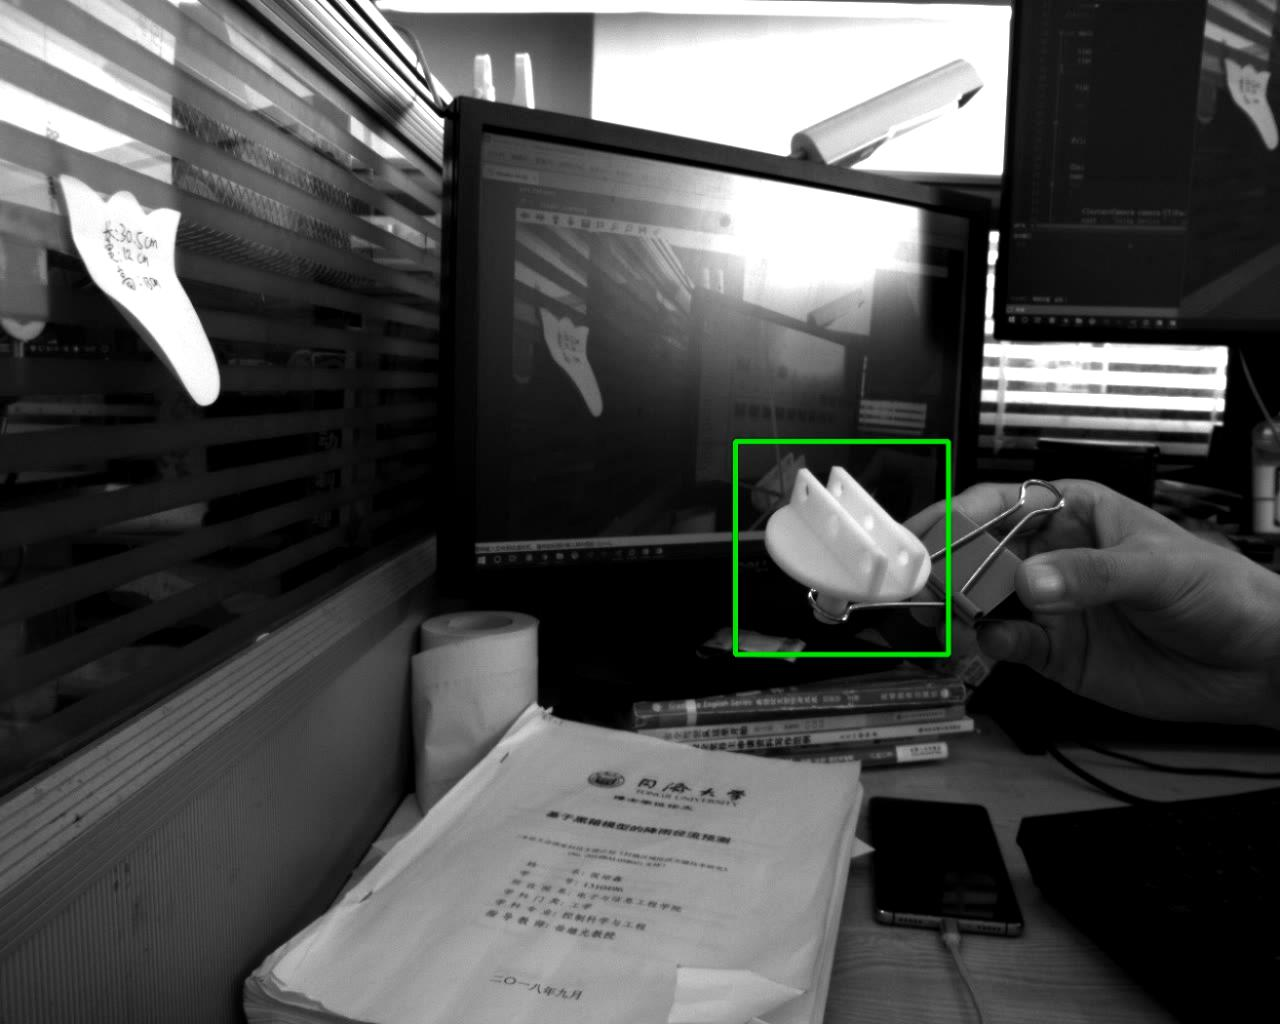
\includegraphics[height=3.8cm]{t_reg_1}
    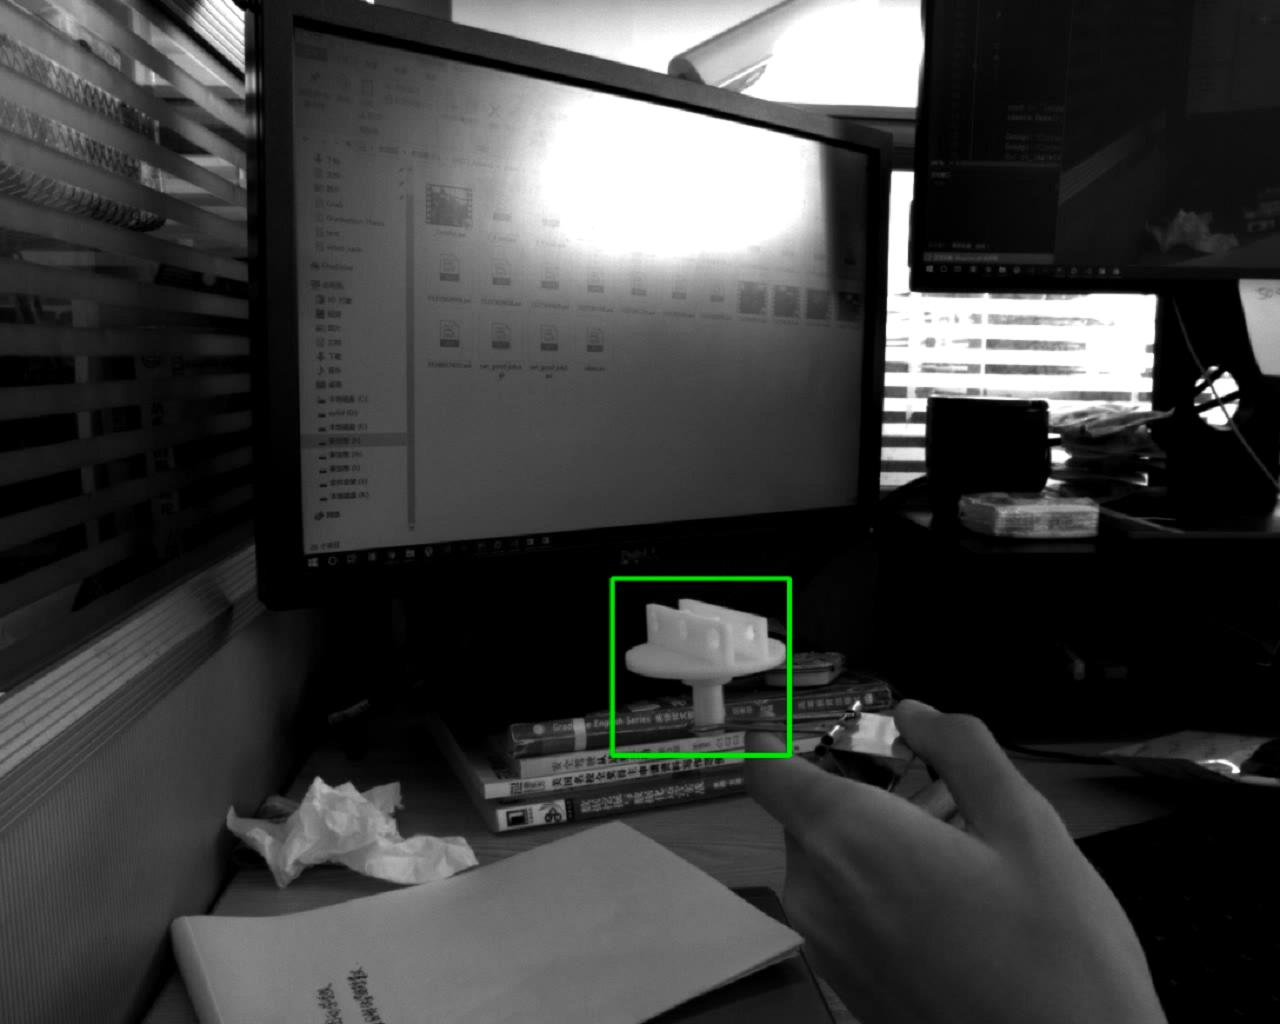
\includegraphics[height=3.8cm]{t_reg_2}
    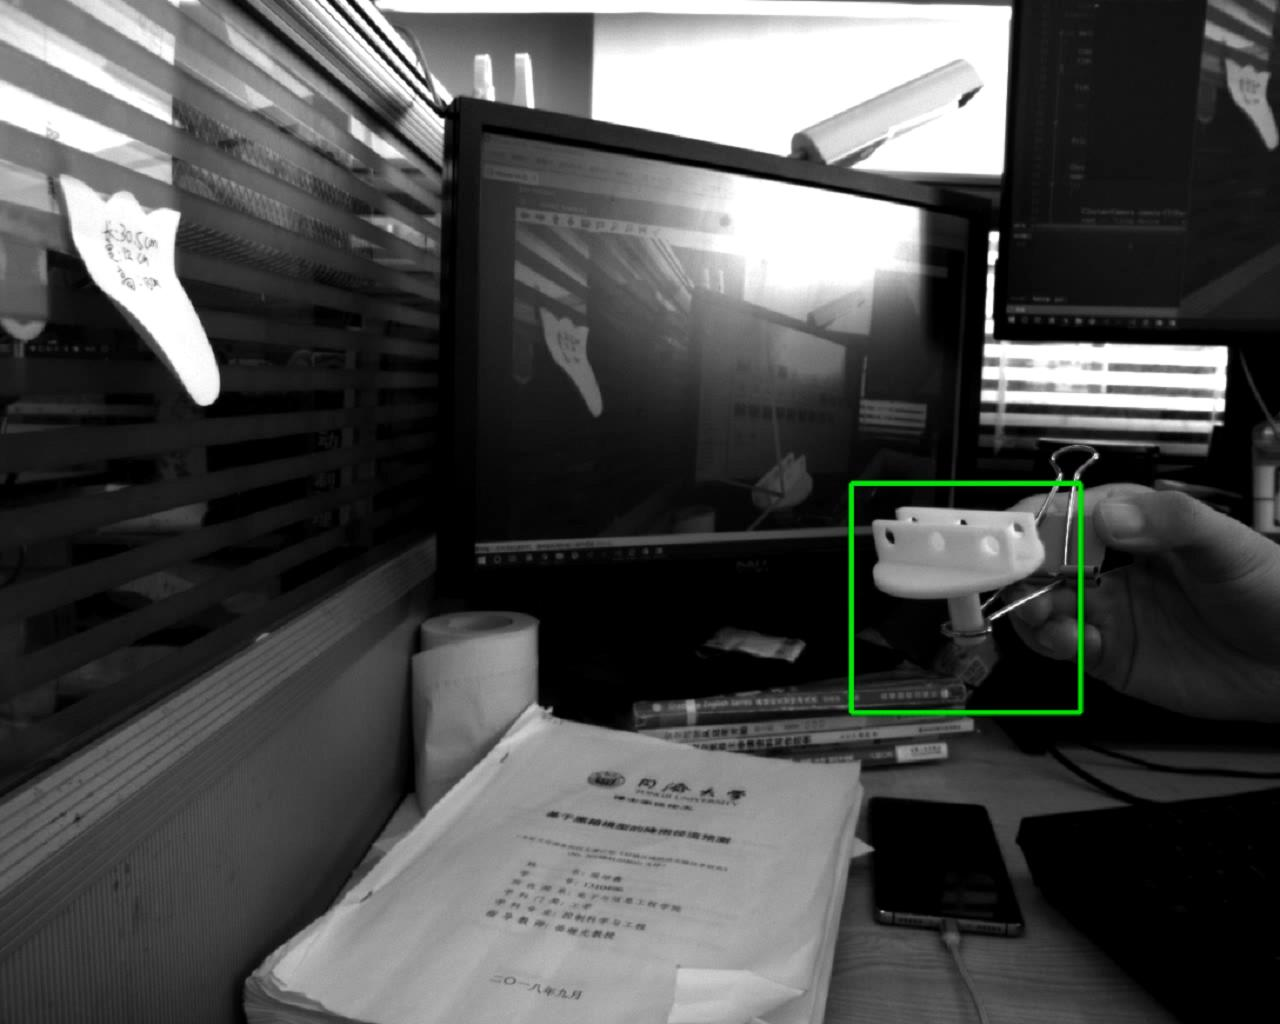
\includegraphics[height=3.8cm]{t_reg_6}
    \quad
    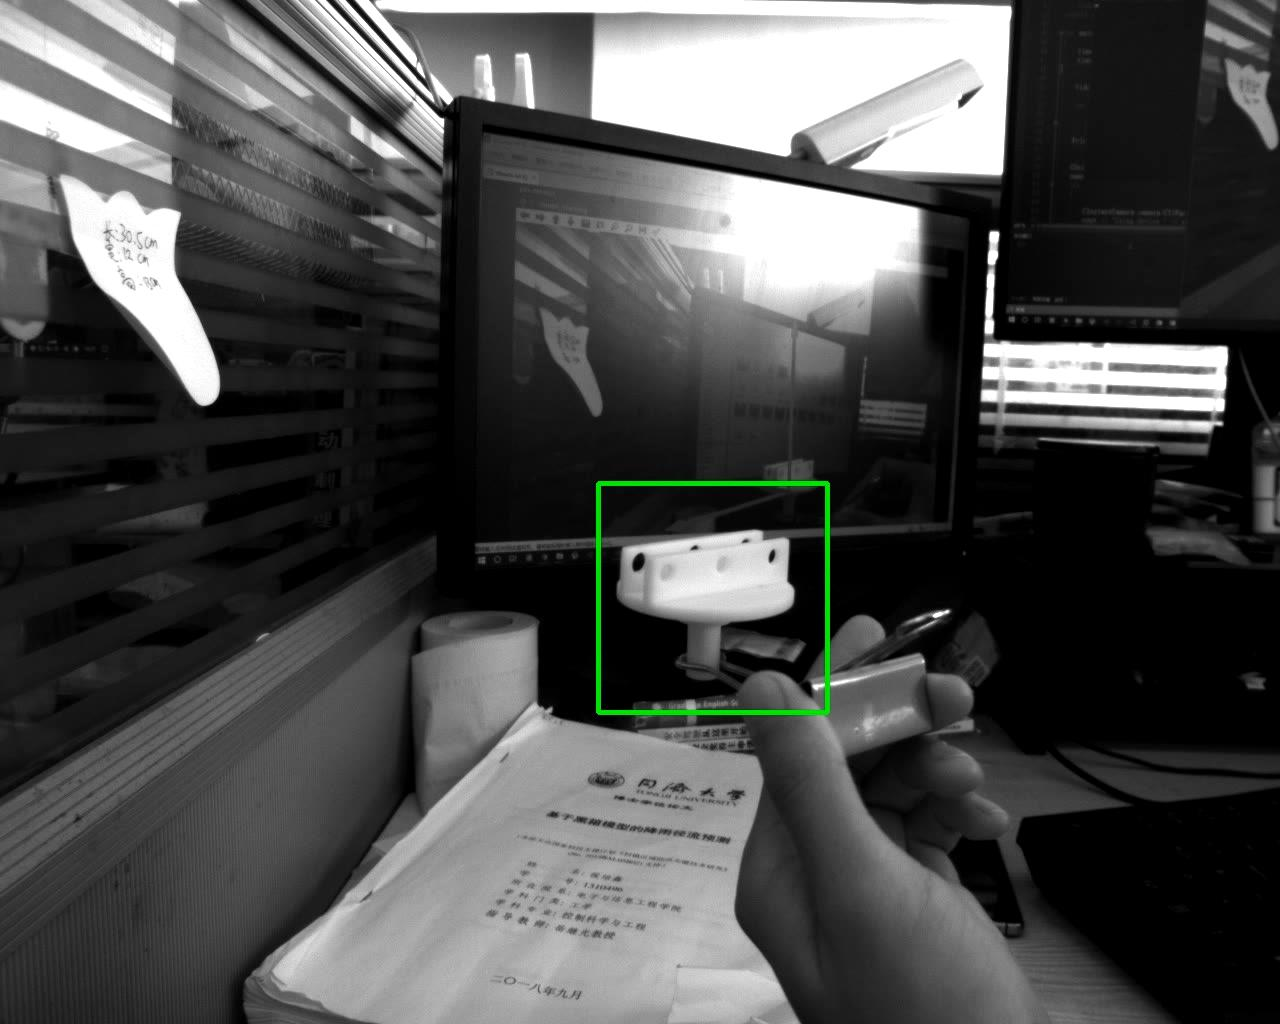
\includegraphics[height=3.8cm]{t_reg_3}
    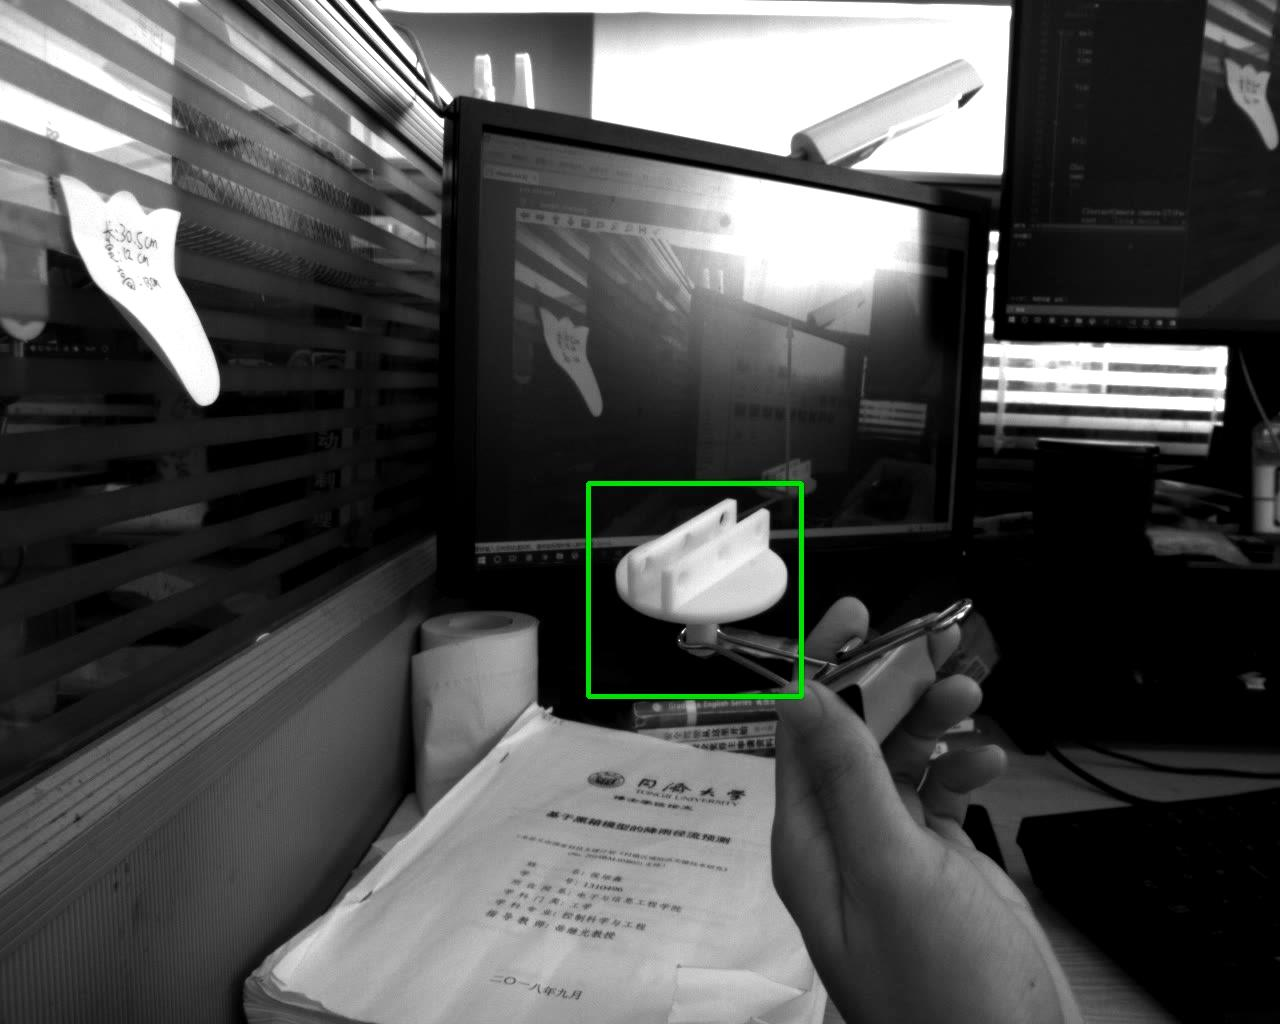
\includegraphics[height=3.8cm]{t_reg_4}
    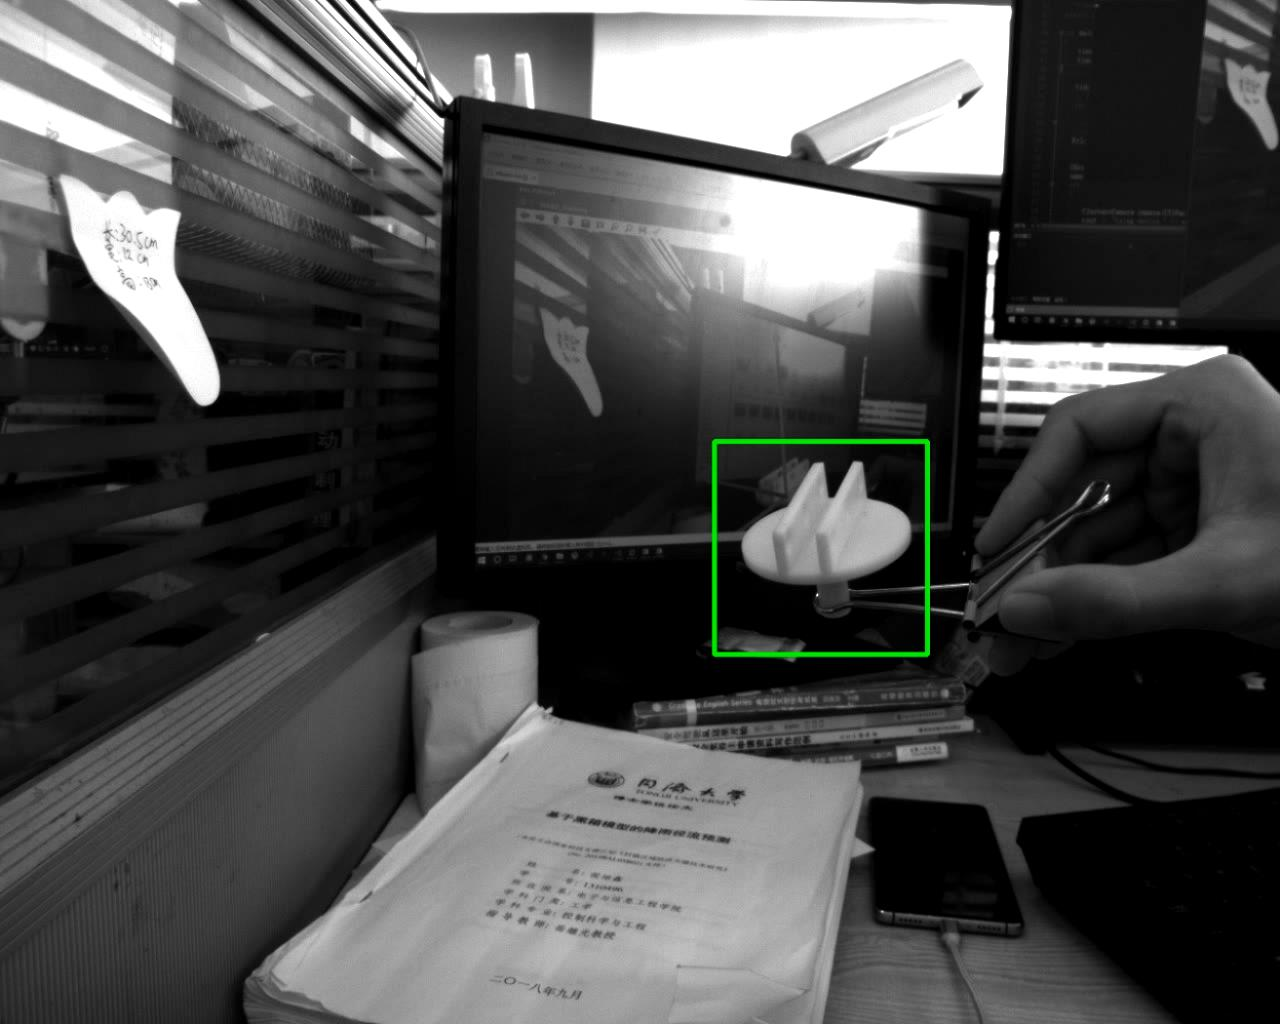
\includegraphics[height=3.8cm]{t_reg_5}
  \caption{多姿态下的目标检测效果图}
    \label{fig:chap04:mul_pose_detect_result}
\end{figure}

\subsection{基于模板匹配的位姿精确估计}
\label{sec:template_pose_accuracy}
完成平移向量估计后,需要获得物体坐标系相对于相机坐标系的旋转关系~$R=[r_x, r_y, r_z]$,其中~$r_x,r_y,r_z$~分别代表绕相机坐标系~$x,y,z$~轴旋转的欧拉角,使用弧度制表示。且欧拉角的旋转顺序为先绕~$x$~轴旋转,后绕
~$y$~轴,最后绕~$z$~轴。旋转顺序不一致将导致结果不同。

本文在检测阶段即对目标物体的姿态进行了粗分类,如图~\ref{fig:chap04:rf_obj_det_pose}~所示,对于不同的目标物体,按照其对称关系分为二分类或者三分类。为获得物体坐标系相对于相机坐标系的精确位姿关系,本文将针对不同
物体的不同粗分类位姿构造姿态模板,通过预先设定多个位姿,寻找当前图片与设定位姿的最优匹配,即通过模板设定的姿态作为前文追踪算法的初始位姿,进行姿态寻优,该过程不仅能够得到精确的旋转向量~$R$,还能进一步提高
通过随机森林回归得到的平移向量~$\textrm{T}$。具体的步骤如算法~\ref{alg:pose_template_match}~所示。
\begin{algorithm}[H]
  \caption{[$R',\textrm{T}'$]=$Match(Q,\textrm{T},T_r,a)$}
  \label{alg:pose_template_match}
  \begin{algorithmic}[1]
    \Require{姿态模板库 $Q$;检测粗分类结果 $a$;平移向量估计结果 $\textrm{T}$;匹配阈值 $T_r$}
    \State 根据粗分类结果选择模板库~$Q_a$.
    \For{$R_t$ \textbf{ in } $Q_a$}
      \State 构造初始化位姿$\{R_t, \textrm{T}\}$.
      \State 使用相机模型与初始化位姿将模型映射到图像平面。
      \State 根据章节~\ref{sec:Objective function Building}~构造优化目标函数。
      \State 根据章节~\ref{sec:Optimization of objective function}~进行位姿配准得到$\{R',\textrm{T}'\}$.
      \State 根据章节~\ref{sec:Direction weight Calculation}~计算配准得分~$T_n$.
      \If{$T_n \geqslant T_r$}
        \State \textbf{Break}
      \EndIf
    \EndFor
    \\
    \Return {$\{R',\textrm{T}'\}$}
  \end{algorithmic}
\end{algorithm}

算法首先通过检测分类的结果在模板库中选择相应的位姿库,之后遍历相应位姿库中的所有姿态~$R_r$~,以联合平移向量~$\textrm{T}$~构造待配准位姿,
最后运行配准优化算法,寻找模板库中的最优匹配,以得到追踪算法的初始化位姿~$\{R',\textrm{T}'\}$。最优匹配的判定标准是根据章节~\ref{sec:Direction weight Calculation}~中提出的光栅点权重计算标准,该标准计算
配准后的模型光栅点边缘方向与场景图像的梯度方向的夹角,以评价配准结果。当配准良好时,模型的边缘方向应与图像的梯度方向垂直,因此计算两个夹角的正弦值~$\alpha~ (0\leq \alpha \leq 1)$~作为该点的得分,
之后平均所有光栅点的得分以得到模型配准的整体得分~$T_n$。当某一个姿态下的得分高于设定的阈值~$T_r$~后,直接返回当前轮循环的~$\{R',\textrm{T}'\}$,而不再继续遍历后续的姿态库。

本文在每一种模型的每一种粗分类位姿下准备了~15~个模板,如图~\ref{fig:chap04:tem_show}~所示为正面粗分类位姿下的部分模板示意图。正面的模板通过等角度间距旋转~$z$~轴得到,遍历正面的~$180^\circ$~角度范围以保证正面的位姿都能够匹配成功,
剩下的~7~个姿态模板通过在粗分类范围内随机生成得到。依靠寻优算法,当待配准姿态与精确姿态相差在~$10^\circ $~以内亦能完成配准,因此允许模板与真实角度有较大角度差异,依靠配准算法能够有效降低模板位姿的数量,
降低算法实现的成本。

本文首先对匹配最近图进行~NPD~特征提取,以训练随机森林对目标物体进行检测,并对其位姿进行粗分类;后以检测的图像位置以及分类结果作为回归树判定的特征,得到目标物体相对于相机坐标系的平移向量;最后通过预设的
位姿模板对图像进行配准,得到精确的位姿关系。随机森林、回归树以及模板的选择都是粗匹配过程,其中可能包含误检以及偏差。如图~\ref{fig:chap04:match_res}~所示,检测阶段的结果可能包含多个检测框,这是由于滑窗的步长选择较小,导致相邻检测框的判定结果都为真,
若扩大滑窗步长,则会导致出现较多的漏检。依靠配准算法能够有效降低前述步骤中产生的误差,且通过章节~\ref{sec:Direction weight Calculation}~中研究的权重计算方法能够对初始化位姿进行
评价,以提高自动初始化算法的可信度,如图~\ref{fig:chap04:match_res}~可知,在多检测结果的干扰下,算法也能够成功获得目标物体相对于相机的初始化位姿(由图中的箭头坐标系可知)。本章研究的算法仅在输入视频的首帧图像中运行,若初始化成功,则将配准后的精准位姿作为追踪算法的初始位姿,实现自动初始化,若初始化失败,则继续处理后续帧图像,直至出现目标物体,并成功初始化。

\begin{figure}[t] %[h]
  \centering%
    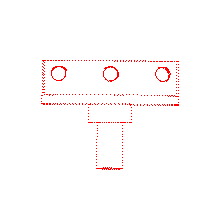
\includegraphics[height=3.5cm]{tmp1}
    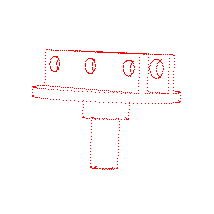
\includegraphics[height=3.5cm]{tmp2}
    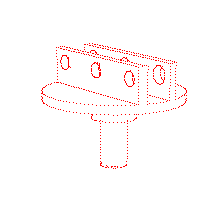
\includegraphics[height=3.5cm]{tmp3}
    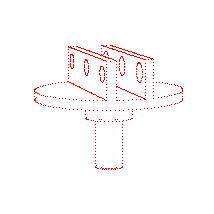
\includegraphics[height=3.5cm]{tmp4}
    \quad
    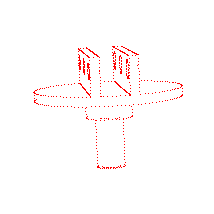
\includegraphics[height=3.5cm]{tmp5}
    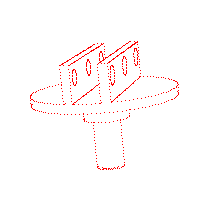
\includegraphics[height=3.5cm]{tmp6}
    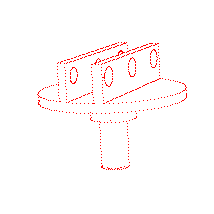
\includegraphics[height=3.5cm]{tmp7}
    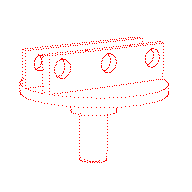
\includegraphics[height=3.5cm]{tmp8}
  \caption{粗分类位姿下的模板示意图}
    \label{fig:chap04:tem_show}
\end{figure}

\begin{figure}[t] %[h]
  \centering%
    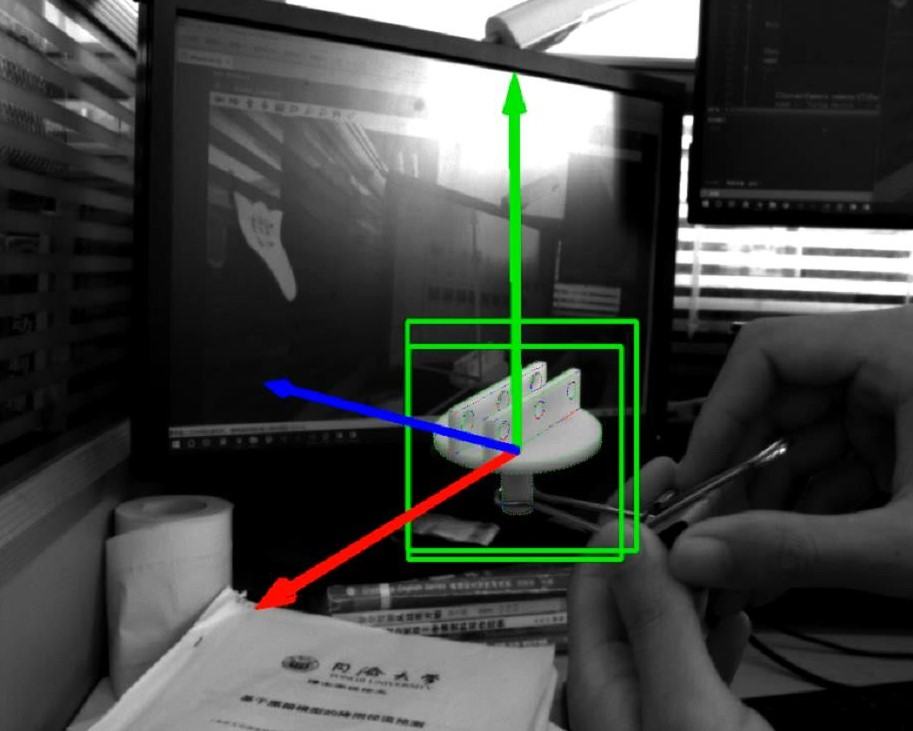
\includegraphics[height=3.8cm]{match1}
    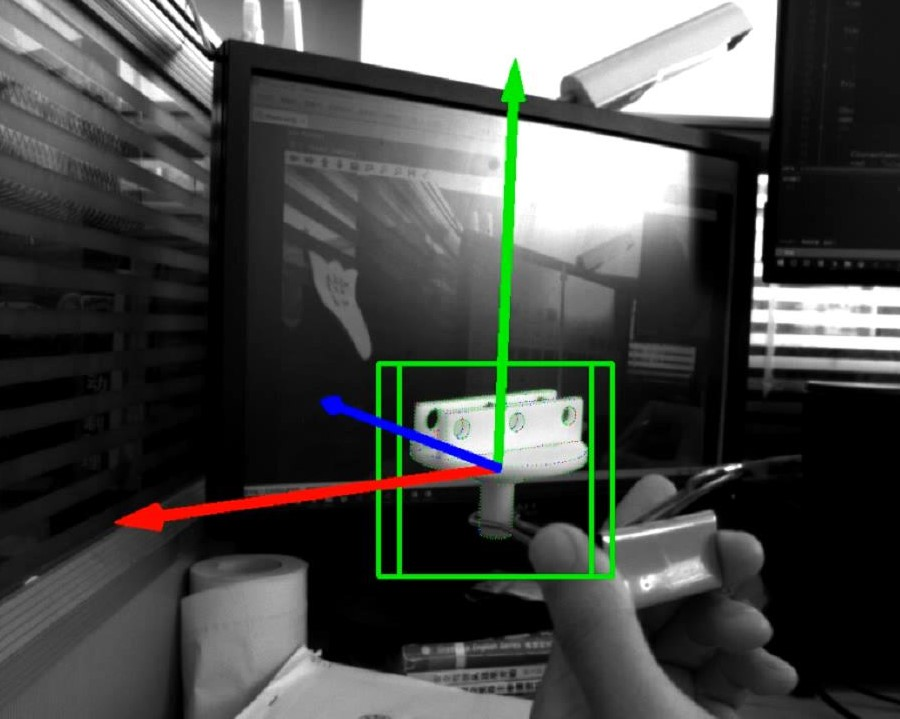
\includegraphics[height=3.8cm]{match2}
    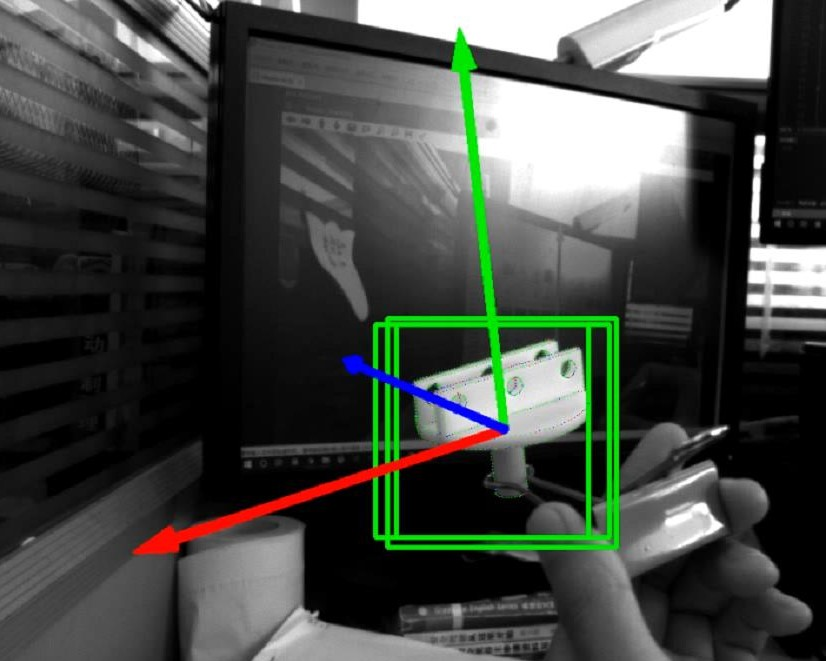
\includegraphics[height=3.8cm]{match4}
  \caption{检测及姿态配准结果示意图}
    \label{fig:chap04:match_res}
\end{figure}

\section{目标检测与追踪系统整合与算法优化}
\label{sec:detect_with_tracking_youhua}
本章研究的检测算法主要是完成物体的图像位置检测及其位姿的估计,其目标是为追踪算法提供精确的初始化位姿,减少人工对齐的成本。得益于本文使用的光栅点权重评价方法,系统能够在追踪过程中检测到追踪失败的情况,该问题主要出现在
目标物体从相机视野中消失,或者出现大面积遮挡等导致追踪算法失效的情况。为提高系统的鲁棒性,本文将利用初始化算法在追踪失败后进行重新初始化。为提高系统的实时性,本节还将研究利用英伟达~GPU~的~CUDA~并行库对算法进行改进以加快速度的方法。

\subsection{目标检测与追踪系统整合}
\label{sec:object_detect_track_union}
目标检测与位姿追踪系统是两个较为独立的系统,目标检测算法通过随机森林以及光栅点匹配的方法在输入图像中寻找目标物体,并估计其相对于相机坐标系的位姿,研究该算法主要是为追踪算法提供初始化位姿,是作为后续追踪
的辅助;而位姿追踪系统是通过给定的位姿或者上帧图像的配准位姿结果作为当前的初始化位姿,之后通过构造光栅点的~DCM~目标函数并寻优,以得到当前帧图像中物体的准确位姿,追踪算法是系统的核心。但追踪算法始终需要上一帧
图像的匹配结果作为初始位姿,该方法将会引进累计误差,当某一帧配准出现较大偏差后,后续的追踪过程将容易出现失效的问题,主要出现在物体消失或者系统出现较大扰动(例如:强光强的过曝、大面积遮挡等)的情况中。为提高系统的鲁棒性,
本文利用光栅点的模型边缘方向与图像梯度方向构建追踪评价得分,具体的方法见章节~\ref{sec:Direction weight Calculation},以判定追踪效果,当出现较大的追踪偏差时,则重新运行检测算法。该策略能够有效应对物体消失后又重新出现的情况,大大提高系统的
稳定性。如图~\ref{fig:chap04:detect_track_flow}~所示为本文所提系统的整体流程图。
\begin{figure}[b] %[h]
  \centering%
    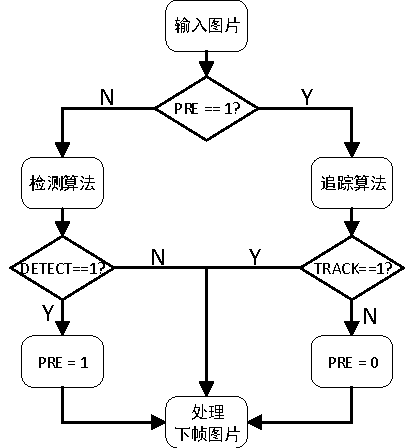
\includegraphics[height=12cm]{track_detect_flow}
  \caption{定位与追踪系统流程图}
    \label{fig:chap04:detect_track_flow}
\end{figure}

其中~PRE~代表算法当前轮处理是否有初始化位姿,若存在,则运行追踪算法,否则运行检测算法。~DETECT~代表是否检测到目标物体并获得其准确的位姿,~TRACK~代表追踪是否成功。当追踪出现较大误差时,算法通过改变
~PRE~的值,使下帧图片输入时运行检测算法,进行重新初始化。
\subsection{加速~DCM~张量计算}
\label{sec:DCM_tensor_cal_speed_up}
检测算法中需要提取场景图片的~DCM~张量以得到匹配最近图,而追踪算法中需要计算~DCM~张量以得到光栅点的残差,构造目标函数。因此本文算法的速度很大程度决定于~DCM~张量的计算速度,而~DCM~张量包含了
各离散方向的倒角匹配图,本文使用等间距的~60~个方向对边缘图像进行离散化,如图~\ref{fig:chap04:60dire_DCM}~所示,该张量的具体介绍见章节~\ref{sec:Tensor calculation}。由于~DCM~张量数据维度较大,若输入灰度图片的尺寸为~800*600,则~DCM~张量中就需要
包含~60*800*600,共计~2880~万个像素点,对于每个像素点都存在较多操作,因此其计算速度非常慢。现有算法已使用~CPU~多线程的方法以求加快张量的计算速度,但对于单张~800*600~的灰度图像,仍需耗时近两秒。
本小节将会研究使用~GPU~的并行计算以加快~DCM~张量计算的方法,以提高检测以及追踪算法的实时性。

图形处理器~(Graphics Processing Unit,缩写:GPU~)~,是一种专门在个人计算机、工作站和一些移动设备上运行绘图运算工作的微处理器。GPU~与CPU~(~Central Processing Unit,中央处理器)~由于设计目标不同,存在较大差异。
它们分别针对了两种不同的应用场景,CPU~需要很强的通用性来处理各种不同的数据类型,同时为保证逻辑判断又会引入大量的分支跳转和中断的处理。这些都使得CPU的内部结构异常复杂。
而GPU面对的则是类型高度统一的、相互无依赖的大规模数据和不需要被打断的纯净的计算环境。因此GPU~不需要复杂的控制逻辑以及优化电路,而采用了数量众多的计算单元,存在更多的线程以及寄存器,能够同时独立地完成更多的任务,
因此其并行计算能力要明显优于~CPU\footnote{节选自:https://en.wikipedia.org/wiki/图形处理器}。

近年来~GPU~发展迅速,由美国英伟达公司发布的最新图灵架构显卡已能够同时拥有上万个线程同时工作。本文研究的~DCM~张量计算过程中,需要操作大量的像素点灰度值,以得到张量的最终结果。
并且计算过程中,各像素点的灰度值相对独立,能够使用并行计算的方法同时获得多个像素点的最终灰度值,显著提高算法的效率。因此本文将利用英伟达公司提出的~CUDA~(Compute Unified Device Architecture,统一计算架构)~对算法进行重写。
首先简要介绍~CUDA~框架的线程模型。CUDA~将~GPU~的线程以网格~(grid)~的方式进行组织,而每个网格中又包含若干个线程块~(block)~,每一个线程块中又包含多个线程,如图~\ref{fig:chap04:cuda_grid_block}~表示一个含有~6~个线程块的
网格,且每个线程块中包含~12~个线程的线程模型。同一个线程块中的众多线程不仅能够并行执行,且能够通过共享存储器的方式实现数据交换,实现能够通信的细粒度并行。而不同线程块之间则不能继续数据交换,因此在不同线程块之间进行不需要通信的粗粒度并行。
粗粒度并行互相之间互不干扰,而细粒度并行则可以通过数据交换实现配合的逻辑。

\begin{figure}[t] %[h]
  \centering%
    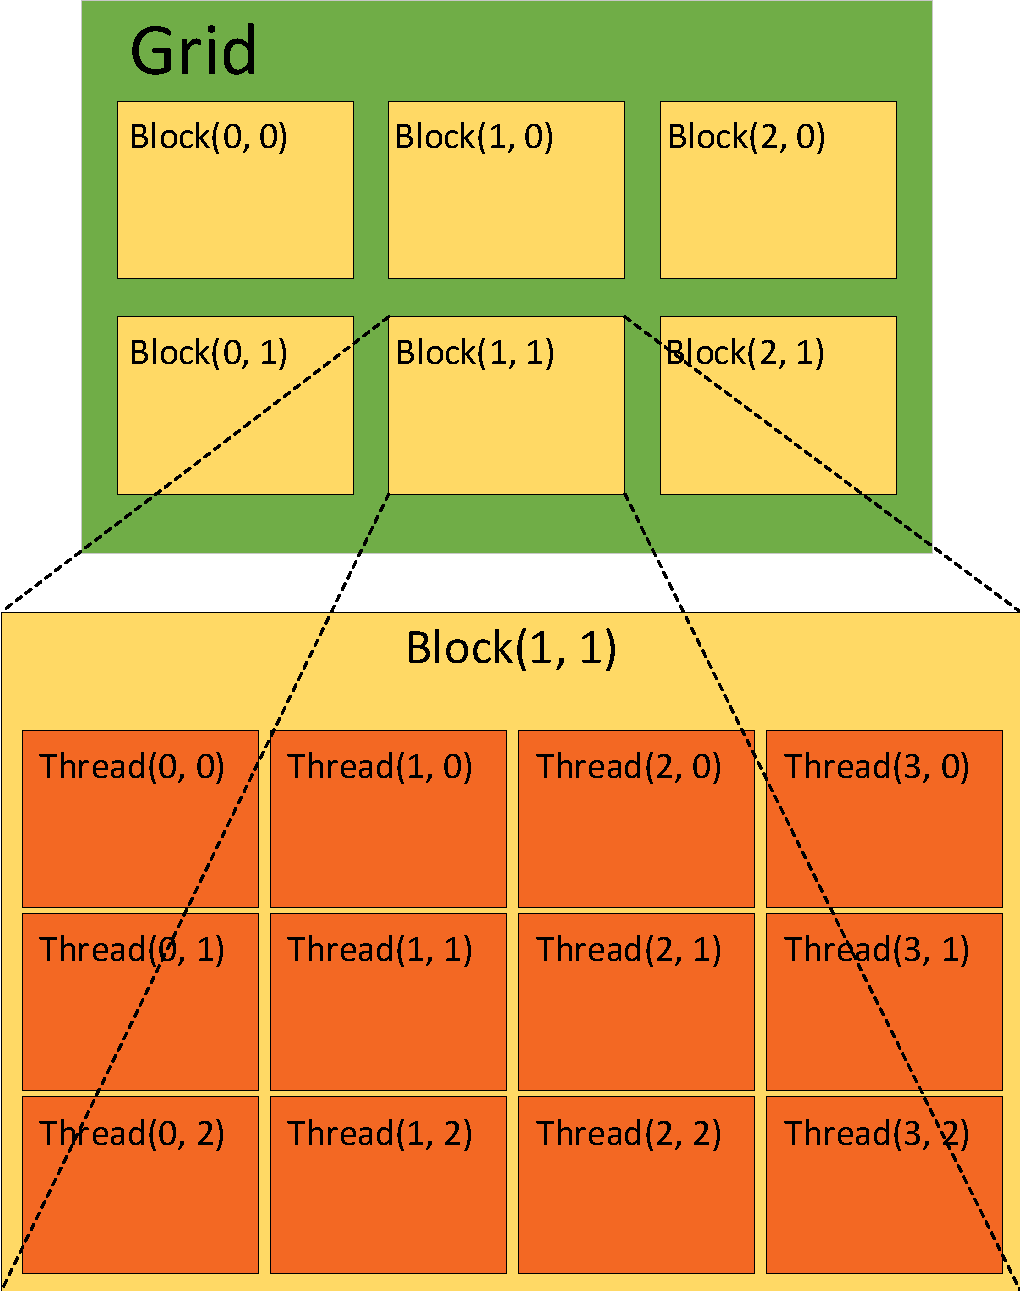
\includegraphics[height=12cm]{cuda_grid_block}
  \caption{CUDA~线程模型}
    \label{fig:chap04:cuda_grid_block}
\end{figure}

DCM~张量的计算过程中,需要对边缘提取以及距离变换后的二维张量图进行双向动态规划,以得到带有角度距离的三维张量图。动态规划算法即计算的后续结果是由当前计算结果决定的。为得到每一个像素点在场景图像中的
最近方向倒角匹配点,算法通过双向遍历的方法,以寻找所有像素点在所有离散方向上的匹配最小值,如式~(\ref{equ:chap04:dp_prog})~所示分别为前向循环以及后向循环的计算方法。对于每一个像素点,需要寻找它在~60~个离散方向上的匹配最近点,
该结果需要循环两次前向循环以及两次后向循环才能找到\footnote{具体证明见:IMPEROLIM,PRETTOA.D2CO:Fast and Robust Registration of 3D Textureless Objects Using the Directional Chamfer Distance}。
这对于包含~2880~万个像素点的~DCM~张量将会产生巨大的计算量。本文在~Inter(R) i7-4790k of 4.00GHZ~的实验平台上使用~CPU~多线程的方法对~800*600~的灰度图像进行~60~个离散方向的~DCM~计算,平均耗时为~83~ms,由于计算过程过慢,极大程度影响
了算法的实时性。为解决该问题,本文将研究使用前述~CUDA~加速方法,对双向动态规划问题进行快速计算。
\begin{equation}
  \label{equ:chap04:dp_prog}
  \left\{
    \begin{aligned}{}
      DT3_V(x,\hat{\phi}_i)=min\{DT3_V(x,\hat{\phi}_i), DT3_V(x,\hat{\phi}_{i-1})+\lambda\lVert \hat{\phi}_{i-1}-\hat{\phi}_{i}\rVert_\pi\}\\
      DT3_V(x,\hat{\phi}_i)=min\{DT3_V(x,\hat{\phi}_i), DT3_V(x,\hat{\phi}_{i+1})+\lambda\lVert \hat{\phi}_{i+1}-\hat{\phi}_{i}\rVert_\pi\}
    \end{aligned}
    \right.
\end{equation}

利用~CUDA~对算法进行加速,关键在于构造~kernal~函数,程序启动后所有线程都将运行该函数,而每个线程处理的输入数据都将不同。假设~width~代表输入图像的像素列数,height~代表输入图像的像素行数,本文构造
线程模型~gridSize~以及~blockSize~如代码~\ref{code:chap4:dp_prog_thread_model}~所示。假设对于~800*600~的灰度图像,构造线程栅格,其中含有~40*30~个线程块,每个线程块中包含~20*20~个线程。构造完成后,
保证一个线程对应一个像素点,线程的坐标对应其需要处理的图像像素点坐标。

由于动态规划过程是在单一像素点的不同方向上进行的,因此不同像素点间的结果互不影响。所以能够构造线程与像素点的一一对应关系,通过大量线程的并行计算,同时得到所有像素点在各离散方向上的最小方向倒角匹配距离,即~DCM~张量,
构造~kernal~函数如代码~\ref{code:chap4:dp_prog_thread_kernal}。
\begin{lstlisting}[
  language=C++,
  numbers=left,                
  numberstyle=\footnotesize,
  frame=single,     
  basicstyle=\small\tt,    
  caption={动态规划线程模型},
  label={code:chap4:dp_prog_thread_model}]
  dim3 gridSize(width / 20, height / 20);
  dim3 blockSize(20, 20);
  \end{lstlisting}
\begin{lstlisting}[
  language=C++,
  numbers=left,                
  numberstyle=\footnotesize,
  frame=single,     
  basicstyle=\small\tt,    
  caption={动态规划过程的~kernal~函数},
  label={code:chap4:dp_prog_thread_kernal}]
  void dy_prog_kernel(float ** data, float ang_p, 
    int num_directions, int width, int height) {
  int col = threadIdx.x + blockIdx.x * 20;
  int row = threadIdx.y + blockIdx.y * 20;
  int index = row * width + col;
  //forward
  for (int loop = 0; loop < 2; ++loop) {
    for (int i = 0; i < num_directions; ++i) {
      int pre_num = (i - 1 == -1) ? num_directions - 1 : i - 1;
      float now = data[i][index];
      float pre = data[pre_num][index];
      float new_data = pre + ang_p;
      data[i][index] = new_data < now ? new_data : now;
    }
  }
  //backward
  for (int loop = 0; loop < 2; ++loop) {
    for (int i = num_directions - 1; i >= 0; --i) {
      int pre_num = (i + 1 == num_directions) ? 0 : i + 1;
      float now = data[i][index];
      float pre = data[pre_num][index];
      float new_data = pre + ang_p;
      data[i][index] = new_data < now ? new_data : now;
    }}}
  \end{lstlisting}

其中函数输入~data~为二维数组,其中保存了所有方向的像素点的二维张量值,完成动态规划后的三维张量值也保存在其中;ang\_p~代表相邻离散角度间的方向差值;num\_directions~代表离散方向的数量。
kernal~函数中首先根据当前的线程块编号以及线程的坐标确定当前线程所有处理的图像像素点坐标~[col,~row],之后再对所选像素点进行双向动态规划,得到该点在各方向上的张量最小值。
本文在~Nvidia(R) GTX 980Ti~的实验平台上使用~CUDA~并行计算的方法对~800*600~的灰度图像进行~60~个离散方向的~DCM~计算,平均耗时为~9~ms,计算速度是~CPU~多线程方法的~10~倍左右。

在完成各像素点的~DCM~张量计算之后,还需要对张量在角度方向上做平滑处理,如式~(\ref{equ:chap04:dt3v_smooth})~所示,以降低边缘提取以及边缘点方向计算的偶然误差对张量的影响,提高匹配的精度。
该过程需要在所有方向的所有像素点上进行计算,因此本文构造三维线程模型,如代码~\ref{code:chap4:smooth_thread}~所示,其中~gridSize~设定为三维线程栅格。假设输入灰度图片的尺寸为~800*600,离散方向的数量为~60,
则该栅格含有~40*30*60~个线程块,每个线程块中包含~20*20~个线程。保证所有离散方向上的像素点都有一个线程与之对应。平滑处理的~kernal~函数如代码~\ref{code:chap4:smooth_kernal}~所示,其中~Pre\_Smooth~为
处理前的数据,After\_Smooth~为处理后的数据。不同于动态规划的~kernal~函数,由于平滑处理中的线程栅格为三维,包含~z~方向上的线程块(本文中使用该方向代表不同的角度方向),通过该方向的序号~blockIdx.z~作为离散角度的
序号,对像素点进行选择,以完成相应像素点灰度值的平滑处理。
\begin{equation}
  \label{equ:chap04:dt3v_smooth}
      DT3_V(x,\hat{\phi}_i) = 0.25 * DT3_V(x,\hat{\phi}_{i-1}) + 0.5 * DT3_V(x,\hat{\phi}_i) + 0.25 * DT3_V(x,\hat{\phi}_{i+1})
\end{equation}
\begin{lstlisting}[
  language=C++,
  numbers=left,                
  numberstyle=\footnotesize,
  frame=single,     
  basicstyle=\small\tt,    
  caption={平滑处理线程模型},
  label={code:chap4:smooth_thread}]
  dim3 gridSize(width / 20, height / 20, num_directions);
  dim3 blockSize(20, 20);
  \end{lstlisting}
\begin{lstlisting}[
  language=C++,
  numbers=left,                
  numberstyle=\footnotesize,
  frame=single,     
  basicstyle=\small\tt,    
  caption={平滑处理的~kernal~函数},
  label={code:chap4:smooth_kernal}]
  void smooth_kernel(float ** Pre_Smooth, float ** After_Smooth, 
    int num, int width, int height) {
  int dir = blockIdx.z;
  int pre_dir = dir - 1 >= 0 ? dir - 1 : num - 1;
  int slow_dir = dir + 1 < num ? dir + 1 : 0;

  int col = threadIdx.x + blockIdx.x * 20;
  int row = threadIdx.y + blockIdx.y * 20;

  int index = row * width + col;
  After_Smooth[dir][index] = 0.25*Pre_Smooth[pre_dir][index] + 
    0.5*Pre_Smooth[dir][index] + 0.25*Pre_Smooth[slow_dir][index];
  }
  \end{lstlisting}

对于~800*600~的灰度图像,设定~60~个离散方向计算~DCM~张量,在前述实验平台中使用~CPU~完成平滑处理的平均耗时为~260~ms,而使用~CUDA~并行计算的耗时仅为~4~ms,提升明显。
\section{本章小结}
\label{sec:chap4:summary}
本章首先研究了基于随机森林的多目标检测方法,对匹配最近图进行~NPD~特征提取,以训练随机森林。设定粗分类位姿,将训练图片按照位姿进行分类,使训练得到的随机森林能够在检测阶段完成同一目标物体的位姿粗分类。
训练完成后,通过滑窗将输入图片进行分割,以使用随机森林对图像的各个区域进行判定。通过该方法能够判定场景图像中是否包含目标物体,若包含,则返回其检测框的图像位置,以及粗分类的类别。

其次,本章继续研究目标物体的精确位姿获取方法。使用检测随机森林得到的检测框信息以及粗分类的类别作为回归森林的训练特征,以估计目标物体相对于相机坐标系的平移向量,本文使用~ranger~随机森林训练库完成该回归森林的
训练,其训练速度以及精度相比其他方法更有优势。之后针对检测结果中的粗分类类别构造姿态匹配模板库,使用姿态模板库以及回归得到的平移向量构造位姿匹配库,通过章节~\ref{sec:Optimization of objective function}~中提出的位姿寻优方法得到当前图片中目标物体的精确位姿,
该位姿用于给追踪算法提供首帧图像中的物体位姿,即初始化位姿,实现自动初始化。

最后,本章研究了目标检测系统与追踪系统的整合,阐述了两个系统互相切换的逻辑,通过模型与边缘图像匹配的评价方法灵活切换两种算法,解决目标物体从相机视野中消失的问题,提高系统的鲁棒性。之后研究~DCM~张量的计算加速方法,使用
显卡的~CUDA~并行计算框架对双向动态规划以及平滑处理进行加速,加速效果显著,大幅提升了算法的实时性。

